\chapter{Methodology}  \label{ch:methodology}

\begin{comment}
Why did I choose my method
\end{comment}

\begin{table}[h]
\centering
 \begin{tabular}{l l} 
 \hline
 SYMBOL & DESCRIPTION \\ 
 \hline
 $K$ & Number of Topics \\  
 $V$ & Number of words in the vocabulary \\
 $M$ & Number of documents \\
 $N$ & Number of words in the document \\
 $N_{d=1..M}$ & Number of words in document d\\
 $\alpha$ & Collection of all $\alpha$ = $ \{ \alpha_{1},\alpha_{2}, ... , \alpha_{K}\}$ \\
 $\alpha_{k=1...K}$ & Hyperparameter for dirichlet prior distribution of topic $k$ \\
 $\beta$ &  Collection of all $\beta$ = $\{\beta{1},\beta{2}, ... , \beta_{K}\}$ \\
 $\beta_{w=1...V}$ & Hyperparameter for dirichlet prior distribution of a word $w$ in a topic \\
 $\varphi_{k=1...K}$ & Distribution of words in topic $k$ \\
 $\varphi_{k=1...K, w=1...V}$ & Weight of  word $w$ in topic $k$  \\
 $\theta{d=1...M}$ & Distribution of topics in document $d$  \\
 $\theta{d=1...M, k=1...K}$ & Weight of  topic $k$ in document $d$ \\
 $z_{d=1...M, w=1...N_d}$ & Assigned topic of word $w$ in document $d$\\
 $Z$ & Topic of all words in documents \\
 $w_{d=1...M, w=...N_d}$ & Assigned word w in document d \\ 
 $W$ & Words in all documents \\ 

 \hline
 \end{tabular}
\caption{Complete notation of LDA}
\label{tab:table1}
\end{table}

\section{Topic Modelling}\label{lda:tm}
Topic models are models used to find latent topics in mostly large unstructured collections of documents. Topic modelling assumes that documents are a mixture of topics, while topics are a distribution of words. \cite{Blei2010}. Where humans have a hard time to find a structure, topic modelling uses statistical methods for analysing words for topic discovery. This makes it possible to compare topics with each other and to find similar documents without necessarily having any prior knowledge of your documents. The application of topic modelling is wide and is very powerful, making it a very popular for exploration of data. 

The machine learning and text mining area have focused a lot on probabilistic topic models in recent years. Models like probabilistic latent semantic analysis (PLSA) and sentiment analysis are used for applications ranging from document clustering, topic modelling and retrieval systems \cite{Lu2011InvestigatingLDA}. Optimising models is a challenging task, making usage of a high range from inference e.g. variational, stochastic variational and Markov chain Monte Carlo \cite{Hoffman2016MarkovModels}. The model that is used in this research and build upon the before mentioned models will be discussed in great length below.


\section{Latent dirichlet allocation}\label{lda:lda}
In natural language processing, \textit{Latent dirichlet allocation} (LDA) is an unsupervised machine learning technique introduced in 2003 for Topic modelling \cite{Blei2003}. The notation used for LDA can be seen in Table \ref{tab:table1}. LDA is part of a larger field called probabilistic topic modelling \cite{Blei2010}.

LDA makes use of a generative probabilistic model of a collection of documents \textbf{M} (corpus) to discover latent topics. Fig \ref{fig:LDA} represents the plate notation of LDA. For a more understandable model consider Fig \ref{fig:LDA_example}. The model assumes that each document \textbf{N} in the corpus consists of a mixture of latent topics. These topics are a mixture of words \textbf{W} assigned to a topic from a fixed vocabulary \textbf{V}. \textbf{Z} notates the assignment of specific words to topics. The distribution of words $\theta$ for each topic is dependent on the sensitivity of $\alpha$. The probability distribution of topics in documents $\varphi$ are depended on the sensitivity of $\beta$. The number of topics \textbf{K} are predefined by the user. 

\begin{figure}
    \centering
    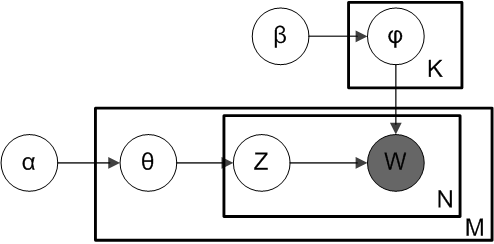
\includegraphics[width=10cm, height=5cm]{methodology/Smoothed_LDA.png}
    \caption{The smoothed LDA plate notation}
    \label{fig:LDA}
\end{figure}

The LDA model is defined in 3 steps and shown in Fig \ref{fig:LDA_example} :
\begin{enumerate}
    \item For each document, pick a topic from its assigned distribution over topics.
    \item Sample a word from the distribution over the words associated with the chosen topic. 
    \item  The process is repeated for all the words in the document.
\end{enumerate}

Let us once again look at the mentioned Fig \ref{fig:LDA_example}. The topics are shown on the left side with their probability of words. On the right side, the document has a topic proportion. Every word gets assigned to a topic so that the topic proportion matches.  
In the original LDA model, assignments of words get updated every iteration through the corpus M. Restarting the process again until the LDA model converges and the topic and assignment are stale. The eventual quality of the model depends on the assumed hyperparameters $\alpha$ and $\beta$ and parameters $\theta$ and $\varphi$. For a better understanding of the parameters take a look at section \ref{lda:alphabeta} and section \ref{lda:thetavarphi}.

\begin{figure}
    \centering
    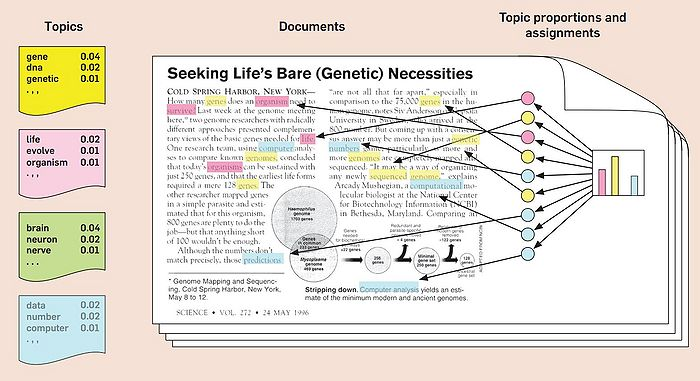
\includegraphics[scale=0.6]{methodology/700px-Illustrating_LDA.jpg}
    \caption{LDA applied to a document}
    \label{fig:LDA_example}
\end{figure}

\subsection{$\alpha$ and $\beta$ hyperparameters}  \label{lda:alphabeta}
The dirichlet is defined as the distribution over a distribution. Dirichlet is used to infer a posterior distribution after observations using a prior distribution \cite{Sethuraman2001APRIORS}. Hyperparameters are defined as parameters that assume a prior distribution before any evidence or information is taken into account. This distinguishes $\alpha$ and $\beta$ from the remaining parameters. $\alpha$ and $\beta$ are both dirichlet distributions. The hyperparameter value $\alpha$ is the parameter of the dirichlet prior on the per-document topic distributions. The result of a high value of $\alpha$ is a document with a mixture of most topics, while the low value leads to documents with more distinct topics. The $\alpha$ results in a corpus with distinct documents or more general documents topic assignments. The value $\beta$ is the parameter of the dirichlet prior of a word in a topic. A high value for $\beta$ means that the topics consists of distinct words, the low value of $\beta$ assumes topics are more generative. The $\beta$ will influence the general distribution of words in topics in the output of topics. We base our $\alpha and \beta$ on earlier research that that $\alpha = 50/T$ with $\beta = 0.01$ works great with many different text collections.

\subsection{$\theta$, $\varphi$ parameters}\label{lda:thetavarphi}
The parameters $\theta, \varphi$ are depend on the prior distributions $\alpha$ and $\beta$. $\theta$ is the document-topic distribution. $\theta$ is the weight of a topic in a document and because $\alpha$ is a prior distribution, $\theta$ assumes a distribution based on the previous assigned distribution. 
In the same way $\varphi$ is the weight of words in a topic. $\varphi$ in this case is dependent on the $\beta$.



\subsection{Online Latent dirichlet allocation} \label{lda:onlinelda}
The online variant of LDA was introduced  by Hoffman et al. in 2010.\cite{Hoffman2010OnlineAllocation} This new variation dealt with the problem earlier LDA models struggled with. The problem that LDA had was the computing of huge collections of documents. The online LDA can be used for massive and streaming documents without losing performance compared to the original LDA model, because it analyses the documents in batches instead of single observations with stochastic (random) optimisation \cite{Beaver2012}. This research also assumes the online model for similar performance and improved computational time.

\subsection{Dimensionality reduction}
The reason LDA is widely applied for text clustering is because LDA actually reduces the dimension, reducing the computation time. Reducing the dimension with LDA allows the usage of Jensen-Shannon distance to measure text similarity, which we discuss in section \ref{research:jsdivergence}. The generated output is also suitable for clustering, but the output can also be interpreted as clusters.

\section{Text preprocessing}
In this section we'll talk about the input dataset, the reason why we selected it and how it got processed for our model. Preprocessing involves tokenization and stop word removal discussed in section \ref{tokenization} - \ref{bagow}. Preprocessing is important and if done wrong can impact the final results. This can be related to the garbage in, garbage out principle in computer science, where flawed input brings nonsense output. 

\subsection{Dataset}
The dataset used in this research is provided by Capgemini containing syslogs from various servers. The syslogs contains event logs from different servers provided to their customers and internal staff. The event logs used on their servers were extracted from different operating systems, ranging from the year 2015 to current day. The size of one day of data can easily range into the 20 - 40 million event logs. Due to the size and complexity and computation time of the dataset, this research contains 1 day of data with the word error to ensure it's associaten with erorrs.
The data will be referred as the corpus and the system logs as documents throughout this research. The corpus contains 426928 records and has messages consisting of small twitter like sizes. The documents has a few features like hostname, severity, port, priority, valid, protocol, body. The features contain little information and will not be used, only the body feature has been extracted which contains the event log.

\subsection{Tokenization}\label{tokenization}
The first step for our preprocessing is the cleaning up of the documents. 
In the preprocessing phase the document needs to be cleaned up and normalised to ensure consistency in the input data.

The content of the document consists of the error message and specific user and server information. An algorithm had to be written to remove the unnecessary information from the dataset. This extracted the message from document and removed the specific users and server information from the message. Afterwards the message got normalised by removing unnecessary punctuation and removing uppercase.

\subsection{Stop word}\label{stop_words}
LDA assumes that each word is equally important, which is simply deduced to not be true from a logical and linguistic point of few. Words such as 'the' and 'a\\an' are not important, generic English words can be removed to only keep the most distinguishable words left. The provided tools in sklearn provide a standard tokenization option with stop words from the English vocabulary. This tool removes remaining ambigious words like single character words and leaves the most important words left that are specific to the error message.

\subsection{Bag of words} \label{bagow}
The text preprocessing in this research makes usage of the bag-of-words representation as LDA makes the assumption that the order of the words does not matter \cite{Blei2010}. Bag of word counts the words that appeared in the document and represent the words in a document as a term frequency matrix. The bag of words representation of a document doesn't take in the order or semantic structure in a document, but LDA discovers these semantic structures itself. 

\begin{comment}

\section{Syslog} 
Syslogs are textual messages \cite{Stearley2004TowardsSyslogs} which contain the messages provided by the systems.


\section{Challenges}

\subsection{Natural Language Processing}


\subsection{Semantics}


\subsection{Sentiment analysis}


\subsection{Extract, Transform, Load}

\end{comment}